%%%------------------------------------------------------------------------------------------------------------
\begin{tikzpicture}
{
\begin{scope}
\node [] (part1label) at (0,0) {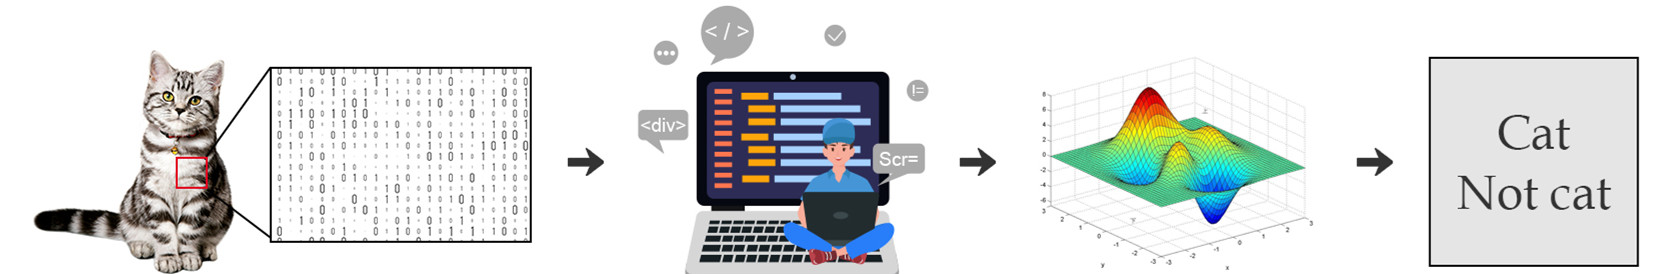
\includegraphics[scale=0.22]{./Chapter9/Figures/figure-feature-engineering.jpg}};
\node [anchor=north,minimum width=2.0em,minimum height=1.5em] (label11) at ([xshift=0.3em,yshift=2em]part1label.north) {\large{特征工程+机器学习}};
\node [anchor=north,minimum width=2.0em,minimum height=1.5em] (label12) at ([xshift=-11em,yshift=-6.3em]part1label.north) {\normalsize{输入}};
\node [anchor=north,minimum width=2.0em,minimum height=1.5em] (label13) at ([xshift=-1em,yshift=-6.3em]part1label.north) {\normalsize{特征提取}};
\node [anchor=north,minimum width=2.0em,minimum height=1.5em] (label14) at ([xshift=6.9em,yshift=-6.3em]part1label.north) {\normalsize{分类}};
\node [anchor=north,minimum width=2.0em,minimum height=1.5em] (label15) at ([xshift=14.2em,yshift=-6.3em]part1label.north) {\normalsize{输出}};
\node [anchor=north,minimum width=2.0em,minimum height=1.5em] (labela) at ([xshift=0.3em,yshift=-8.3em]part1label.north) {\small{(a)基于特征工程的机器学习方法做图像分类}};
\end{scope}
}
{
\begin{scope}[yshift=-1.9in]
\node [] (part1label2) at (0,0) {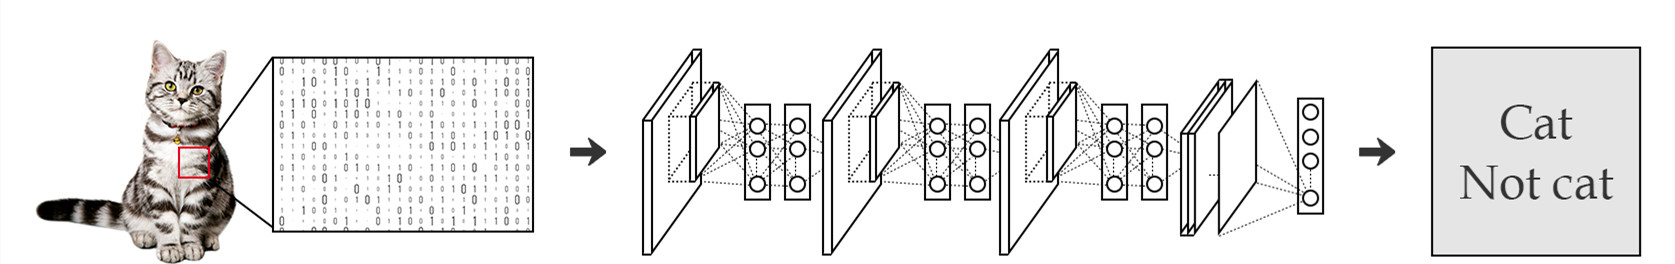
\includegraphics[scale=0.22]{./Chapter9/Figures/figure-deep-learning.jpg}};
\node [anchor=north,minimum width=2.0em,minimum height=1.5em] (label21) at ([xshift=0.2em,yshift=1.2em]part1label2.north) {\large{深度学习(端到端学习)}};
\node [anchor=north,minimum width=2.0em,minimum height=1.5em] (label22) at ([xshift=-11em,yshift=-6em]part1label2.north) {\normalsize{输入}};
\node [anchor=north,minimum width=2.0em,minimum height=1.5em] (label23) at ([xshift=3.0em,yshift=-6em]part1label2.north) {\normalsize{特征提取+分类}};
\node [anchor=north,minimum width=2.0em,minimum height=1.5em] (label24) at ([xshift=14.2em,yshift=-6em]part1label2.north) {\normalsize{输出}};
\node [anchor=north,minimum width=2.0em,minimum height=1.5em] (labelb) at ([xshift=0.3em,yshift=-8em]part1label2.north) {\small{(b)端到端学习方法做图像分类}};
\end{scope}
}
\end{tikzpicture}
%%%------------------------------------------------------------------------------------------------------------
